\subsubsection{Results}

In order to evaluate the model, train, test, max k (max number of clusters) are passed to the function along with where to save the results. In our case, we are using silhouette score to measure cluster performance. In the function bellow, we are creating scores (from create model function) for different number of clusters. At the end we append score to the list which is then used in order to plot the silhouette score.
\begin{listing}[H]
\caption{Evaluate kmeans model}
\begin{minted}{python}
def evaluate_kmeans_model(train_df, test_df, max_k, file_Path):
    silhouette_scores = []

    for k in range(2, max_k + 1):
        predictions = create_kmeans_model(train_df, test_df, k)

        evaluator = ClusteringEvaluator()

        silhouette = evaluator.evaluate(predictions)

        silhouette_scores.append(silhouette)

    plt.plot(range(2, max_k + 1), silhouette_scores, marker='o')
    plt.xlabel('Number of Clusters (k)')
    plt.ylabel('Silhouette Score')
    plt.title('Silhouette Score vs. Number of Clusters')

    plt.savefig(file_Path)

    plt.close()
\end{minted}
\end{listing}

\begin{figure}[H]
    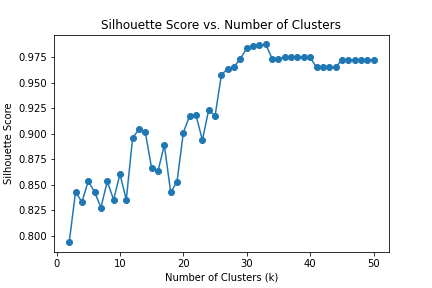
\includegraphics[scale=0.85]{img/Model/Clustering/kmenas.png}
    \centering
    \caption{Silhouette k-means}
    \label{fig:SVM_confusion_matrix}
\end{figure}